\documentclass[12pt,a4paper]{article}

\usepackage[utf8]{inputenc}
\usepackage[T2A]{fontenc}
\usepackage[russian]{babel}
\usepackage{amsmath,amssymb}
\usepackage{graphicx}
\usepackage{booktabs}
\usepackage{multirow}
\usepackage{geometry}
\usepackage{float}
\usepackage{eso-pic}
\graphicspath{{./}}

\geometry{top=2cm,bottom=2cm,left=2.5cm,right=1.5cm}




\title{\textbf{Лабораторная работа 1.3.2}\\
Определение модуля кручения}

\author{
    Студент \underline{Шеховцов Василий Максимович}\\
    Группа \underline{Б03-601}\\
    Преподаватель \underline{Ивлев Д.А.}
}

\date{
Московский Физико-технический институт\\
(национальный исследовательский университет)\\
30 сентября 2026 г.
}

\begin{document}

\AddToShipoutPictureFG*{
    \AtPageUpperLeft{
        \hspace{1.5cm}
        \raisebox{-1cm}{
            \makebox[0pt][l]{Шеховцов В.М.}
        }
    }
}

\maketitle

\section{Аннотация}

\textbf{Цель работы:} измерение углов закручивания в зависимости от приложенного момента сил, расчёт модулей кручения и сдвига
при статическом закручивании стержня, определение тех же модулей для проволоки по измерениям периодов крутильных
колебаний подвешенного на ней маятника (динамическим методом).

\textbf{Оборудование.} Первая часть: исследуемый стержень, отсчётная труба со шкалой, рулетка, микрометр, набор грузов.
Вторая часть: проволока из исследуемого материала, грузы, секундомер, микрометр, рулетка, линейка.

\section{Теоретические сведения}

При закручивании цилиндрических стержней круглого сечения распределение
деформаций и напряжений одинаково по длине стержня только вдали от мест,
где прикладываются закручивающие моменты. Для этих областей можно считать,
что каждое поперечное сечение поворачивается как жёсткое, то есть частички
материала не сходят с тех радиальных линий, на которых они находились вначале,
и все эти радиальные линии поворачиваются на один и тот же угол. Такое напряжённое
состояние называется чистым кручением.

При такой деформации любая прямая линия, проведённая до закручивания цилиндра по частицам
материала и параллельная оси симметрии, превращается в спираль (винтовую линию), как показано на рис.~\ref{fig:torsion}.

\begin{figure}[H]
    \centering
    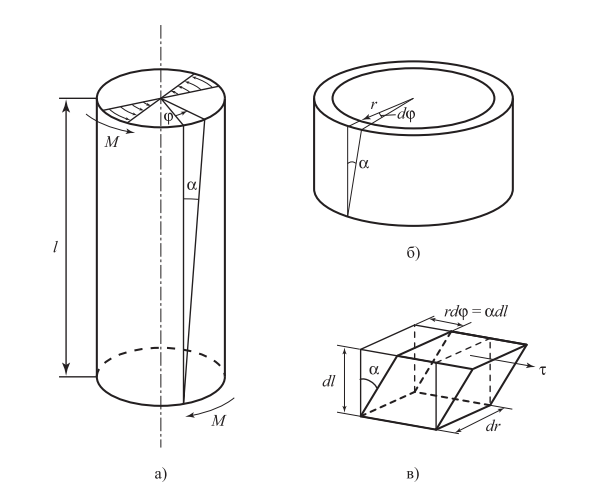
\includegraphics[width=0.8\textwidth]{map1.png}
    \caption{Закручивание цилиндра}
    \label{fig:torsion}
\end{figure}

Покажем, что касательное напряжение в поперечном сечении увеличивается пропорционально расстоянию до оси вращения.
Рассмотрим в цилиндре колечко радиуса $r$ с бесконечно малой толщиной $dr$ и высотой $dl$.
При закручивании верхнее сечение колечка поворачивается относительно нижнего на угол $d\varphi$,
а образующая наклоняется на угол $\alpha$. Тогда при малых углах справедливо соотношение
\begin{equation}
    \alpha\,dl = r\,d\varphi.
    \label{eq:alpha}
\end{equation}
Касательное напряжение $\tau$ связано с углом $\alpha$ линейной зависимостью через модуль сдвига $G$, и, следовательно,
растёт с увеличением расстояния от оси:
\begin{equation}
    \tau = G\alpha = G r \frac{d\varphi}{dl}.
    \label{eq:tau}
\end{equation}
Эти касательные напряжения создают момент сил относительно оси цилиндра:
\begin{equation}
    dM = 2\pi r\,dr\cdot r\cdot\tau.
\end{equation}
Интегрируя это выражение по всем колечкам от оси цилиндра до его радиуса $R$, находим суммарный момент сил:
\begin{equation}
    M = 2\pi G \frac{d\varphi}{dl}\int_0^R r^3\,dr = \frac{\pi G R^4}{2}\frac{d\varphi}{dl}.
    \label{eq:M_int}
\end{equation}
Так как момент сил не меняется по длине цилиндра, для связи приложенного момента $M$ и угла поворота $\varphi$
поперечных сечений, находящихся на расстоянии $l$, имеем
\begin{equation}
    M = \frac{\pi R^4 G}{2l}\,\varphi = f\varphi,
    \label{eq:M_f}
\end{equation}
где $f$ --- модуль кручения, связанный с модулем сдвига $G$ соотношением
\begin{equation}
    G = \frac{2l}{\pi R^4}\,f = \frac{32\,l}{\pi d^4}\,f.
    \label{eq:G}
\end{equation}
Зависимость \eqref{eq:M_f} выполняется при напряжениях, намного меньших модуля сдвига, то есть при малых углах $\alpha$.

\textbf{Статический метод.} Закручивающий момент создают две нити, навитые на шкив диаметром $D$, к концам которых подвешены
одинаковые грузы массой $m$. Две силы $mg$ образуют пару сил, поэтому
\begin{equation}
    M = mgD.
    \label{eq:M_static}
\end{equation}
Угол закручивания находится по смещению $\Delta l$ изображения шкалы в зрительной трубе. При повороте зеркальца на угол $\varphi$
отражённый луч поворачивается на $2\varphi$, поэтому при малых углах
\begin{equation}
    \varphi = \frac{\Delta l}{2L},
    \label{eq:phi}
\end{equation}
где $L$ --- расстояние от зеркальца до шкалы.

\textbf{Динамический метод.} В системе можно возбудить крутильные колебания. Вращение стержня с закреплёнными на нём грузами
вокруг вертикальной оси происходит под действием упругого момента $M$. С учётом выражения для момента получим уравнение колебаний
\begin{equation}
    I\frac{d^2\varphi}{dt^2} + f\varphi = 0.
    \label{eq:osc}
\end{equation}
Следовательно, период колебаний системы связан с расстоянием $r$ от оси вращения до центров масс грузов и моментом
инерции стержня $I_0$ следующим образом:
\begin{equation}
    T^2 = (2\pi)^2\frac{I}{f} = (2\pi)^2\frac{I_0}{f} + (2\pi)^2\frac{m_1+m_2}{f}\,r^2.
    \label{eq:T2}
\end{equation}
Эти зависимости получены для незатухающих колебаний. Поэтому для их применения необходимо убедиться, что в рассматриваемой системе
диссипативными силами можно пренебречь. Для этого стоит убедиться, что период колебаний не зависит от начальной амплитуды
и что амплитуда уменьшается не более чем в 2 раза после около 10 колебаний.

\section{Экспериментальная установка}

\textbf{Статический метод.} Верхний конец вертикально расположенного стержня жёстко закреплён на стойке, а нижний соединён с диском.
Момент, закручивающий стержень, создают две навитые на диск и перекинутые через блоки нити, к концам которых подвешиваются одинаковые грузы.
Диск снабжён зеркальцем: зрительная труба направлена на него, и в неё видно отражение шкалы. Измерение смещения изображения шкалы
позволяет определить угол закручивания (рис.~\ref{fig:static}).

\begin{figure}[H]
    \centering
    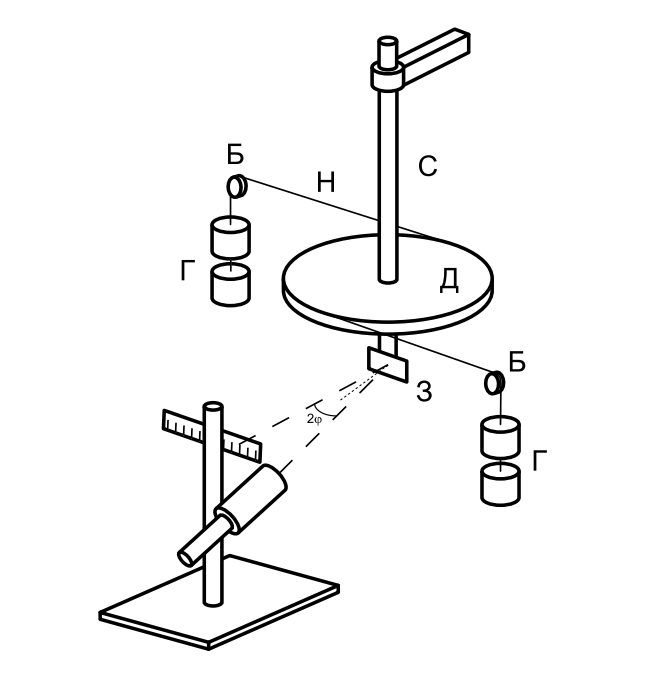
\includegraphics[width=0.6\textwidth]{map2.png}
    \caption{Схема установки для статического закручивания стержня}
    \label{fig:static}
\end{figure}

\textbf{Динамический метод.} Установка состоит из длинной вертикально висящей проволоки, к нижнему концу которой прикреплён
горизонтальный металлический стержень с двумя симметрично расположенными грузами. Положение грузов на стержне можно фиксировать.
Верхний конец проволоки зажат в цангу и вместе с ней может поворачиваться вокруг вертикальной оси. Таким способом в системе
возбуждаются крутильные колебания (рис.~\ref{fig:dynamic}).

\begin{figure}[H]
    \centering
    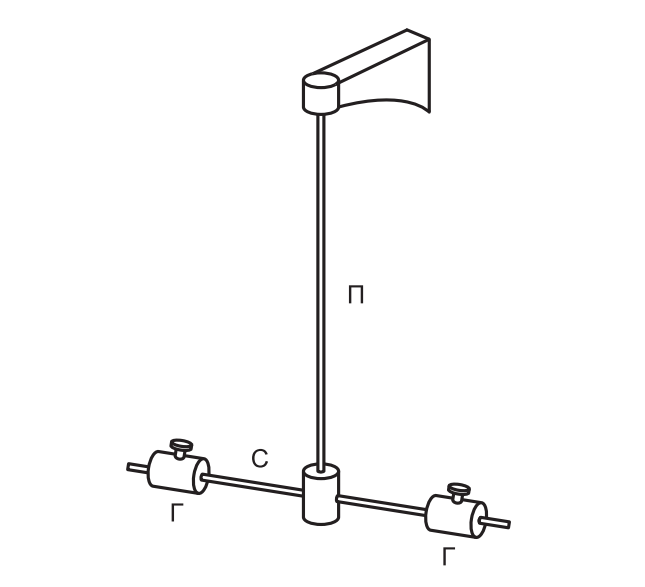
\includegraphics[width=0.6\textwidth]{map3.png}
    \caption{Схема установки для измерения периода крутильных колебаний}
    \label{fig:dynamic}
\end{figure}

\section{Результаты эксперимента и обработка данных}

\subsection{Часть I. Статический метод}

\begin{itemize}
    \item Установим параметры системы. Диаметр стержня штангенциркулем при всех измерениях составлял 0.60 см.
    \[
        D = 10.46 \pm 0.06~\text{см}, \quad d = 0.60 \pm 0.005~\text{см}, \quad l = 175.0 \pm 0.2~\text{см}, \quad L = 148.5 \pm 0.1~\text{см},
    \]
    \[
        \varepsilon_D = 0.6\%, \qquad \varepsilon_d = 0.8\%, \qquad \varepsilon_l = 0.1\%, \qquad \varepsilon_L = 0.1\%.
    \]
    

    \item Увеличиваем нагрузку ступенями, затем уменьшаем в обратном порядке; всего три серии. Масса $m$ --- масса груза на одной нити,
    $\Delta l$ --- отсчёт по шкале в см. При массе 50 г показания шкалы приняты за начальные. Результаты в таблице~\ref{tab:static_data}: до горизонтальной черты --- нагружение, после неё --- разгрузка.

    \begin{table}[!htb]
        \centering
        \caption{Измерения при статическом закручивании}
        \label{tab:static_data}
        \begin{tabular}{c|ccc}
            \toprule
            $m$, г & $\Delta l_1$, см & $\Delta l_2$, см & $\Delta l_3$, см \\
            \midrule
            50  & $-0.10$ & 0.10 & 0.10 \\
            100 & 2.30 & 2.50 & 2.30 \\
            150 & 5.20 & 4.90 & 5.10 \\
            200 & 7.45 & 7.90 & 7.70 \\
            250 & 10.10 & 10.30 & 9.90 \\
            300 & 12.90 & 13.10 & 13.00 \\
            400 & 17.60 & 18.00 & 18.50 \\
            500 & 23.80 & 23.40 & 23.90 \\
            \midrule
            400 & 18.00 & 18.10 & 18.00 \\
            300 & 12.80 & 13.10 & 12.80 \\
            250 & 10.30 & 9.80 & 10.40 \\
            200 & 7.40 & 7.90 & 7.60 \\
            150 & 5.20 & 5.10 & 5.10 \\
            100 & 2.60 & 2.50 & 2.30 \\
            50  & $-0.05$ & 0.20 & $-0.10$ \\
            \bottomrule
        \end{tabular}
    \end{table}

    \item Момент сил и угол закручивания вычисляем по формулам \eqref{eq:M_static} и \eqref{eq:phi}. Максимальные значения
    $M_{\max} = 0.513$ Н$\cdot$м, $\varphi_{\max} = 0.0805$ рад, то есть углы малы. По всем 45 точкам строим график зависимости $M(\varphi)$ методом
    наименьших квадратов (рис.~\ref{fig:static_graph}). Нагружение и разгрузка лежат на одной прямой, поэтому остаточных деформаций и заметного трения в блоках нет.

    \begin{figure}[H]
        \centering
        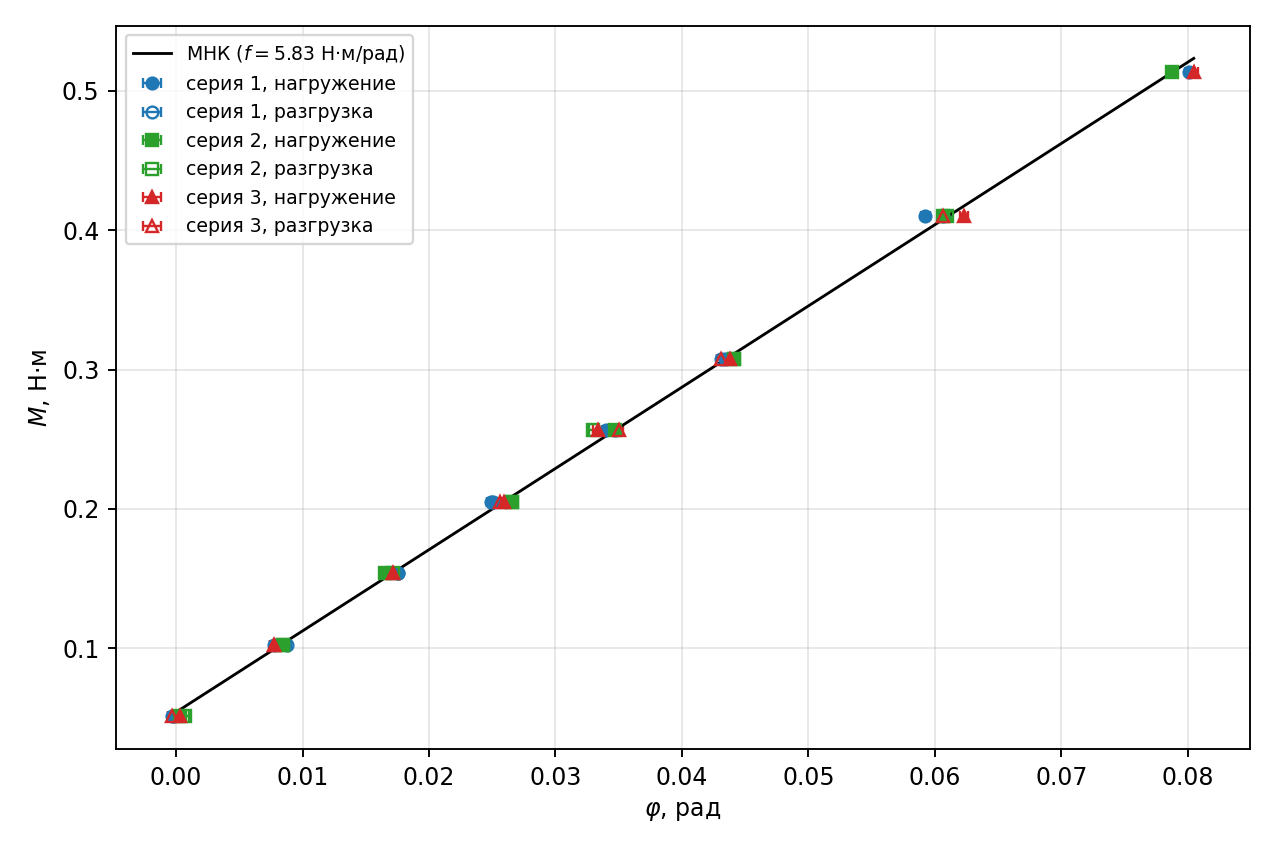
\includegraphics[width=0.85\textwidth]{graph_static.png}
        \caption{Зависимость момента $M$ от угла закручивания $\varphi$}
        \label{fig:static_graph}
    \end{figure}

    \item Коэффициент наклона графика (модуль кручения) определяем по формулам МНК ($N=45$):
    \[
        f = \frac{\langle M\varphi\rangle - \langle M\rangle\langle\varphi\rangle}{\langle\varphi^2\rangle - \langle\varphi\rangle^2} = 5.83~\text{Н}\cdot\text{м/рад},
    \]
    \[
        \varepsilon_f^{\text{случ}} = \frac{1}{f\sqrt{N-2}}\sqrt{\frac{\langle M^2\rangle - \langle M\rangle^2}{\langle\varphi^2\rangle - \langle\varphi\rangle^2} - f^2} = 0.5\%,
        \qquad
        \varepsilon_f^{\text{сист}} = \sqrt{\varepsilon_D^2 + \varepsilon_L^2} = 0.6\%,
    \]
    \[
        \varepsilon_f = \sqrt{\left(\varepsilon_f^{\text{случ}}\right)^2 + \left(\varepsilon_f^{\text{сист}}\right)^2} = 0.8\%, \qquad f = (5.83 \pm 0.04)~\text{Н}\cdot\text{м/рад}.
    \]

    \item Модуль сдвига находим по формуле \eqref{eq:G}:
    \[
        G = \frac{32\,l}{\pi d^4}\,f = 80.1~\text{ГПа}, \qquad
        \varepsilon_G = \sqrt{\varepsilon_f^2 + \varepsilon_l^2 + 16\varepsilon_d^2} = 3.4\%,
    \]
    \[
        G = (80.1 \pm 2.7)~\text{ГПа}.
    \]
    Основной вклад в погрешность даёт диаметр стержня, так как он входит в четвёртой степени.
\end{itemize}

\subsection{Часть II. Динамический метод}

\begin{itemize}
    \item Перед началом работы установим параметры системы.
    \[
        l = 175.0 \pm 0.2~\text{см}, \quad d = 1.473 \pm 0.007~\text{мм}, \quad m_1 = 377.5 \pm 0.05~\text{г}, \quad m_2 = 373.1 \pm 0.05~\text{г},
    \]
    \[
        \varepsilon_l = 0.1\%, \qquad \varepsilon_d \approx 0.5\%, \qquad \varepsilon_{m_1} = \varepsilon_{m_2} = 0.01\%.
    \]


    \item Закрепим грузы на некотором расстоянии от оси и возбудим крутильные колебания. Перед началом измерений убедимся, что выбран правильный диапазон
    амплитуд, в котором можно пренебречь затуханием и применять уравнения гармонических колебаний. Период измерен при двух начальных амплитудах
    (одно деление шкалы --- 1 см), результаты в таблице~\ref{tab:amp}.

    \begin{table}[H]
        \centering
        \caption{Зависимость периода от начальной амплитуды}
        \label{tab:amp}
        \begin{tabular}{|c|c|c|c|}
            \hline
            Амплитуда, см & $t$, с & $N$ & $T = t/N$, с \\
            \hline
            10 & 81 & 22 & 3.68 \\
            \hline
            25 & 113 & 31 & 3.65 \\
            \hline
        \end{tabular}
    \end{table}

    Периоды при разных амплитудах совпадают в пределах погрешности (различие около 1\%), то есть период от амплитуды не зависит.
    Колебания наблюдались в течение 22 и 31 периода, при этом за 10 периодов амплитуда уменьшалась менее чем в 2 раза, поэтому затуханием можно пренебречь.
    Для дальнейших измерений выбрана амплитуда 20 см.

    \item Убедившись в том, что затуханием можно пренебречь, установим грузы на стержне на одинаковом расстоянии $r$ от оси системы до центров масс грузов.
    Будем измерять период $T$ в зависимости от $r$ и занесём данные в таблицу~\ref{tab:dyn}.

    \begin{table}[H]
        \centering
        \caption{Измерение периода в зависимости от расстояния $r$}
        \label{tab:dyn}
        \begin{tabular}{|c|c|c|c|}
            \hline
            $r$, см & $T$, с & $r^2$, см$^2$ & $T^2$, с$^2$ \\
            \hline
            3 & 2.05 & 9 & 4.20 \\
            4 & 2.25 & 16 & 5.06 \\
            6 & 2.80 & 36 & 7.84 \\
            8 & 3.40 & 64 & 11.56 \\
            9 & 3.65 & 81 & 13.32 \\
            10 & 3.90 & 100 & 15.21 \\
            \hline
        \end{tabular}
    \end{table}

    \item По полученным данным строим график зависимости $r^2$ от $T^2$ методом наименьших квадратов (рис.~\ref{fig:dyn_graph}).
    По величине наклона определяем модуль кручения и его погрешность. Принятые погрешности: $\sigma_T = 0.02$ с, $\sigma_r = 0.1$ см.

    \begin{figure}[H]
        \centering
        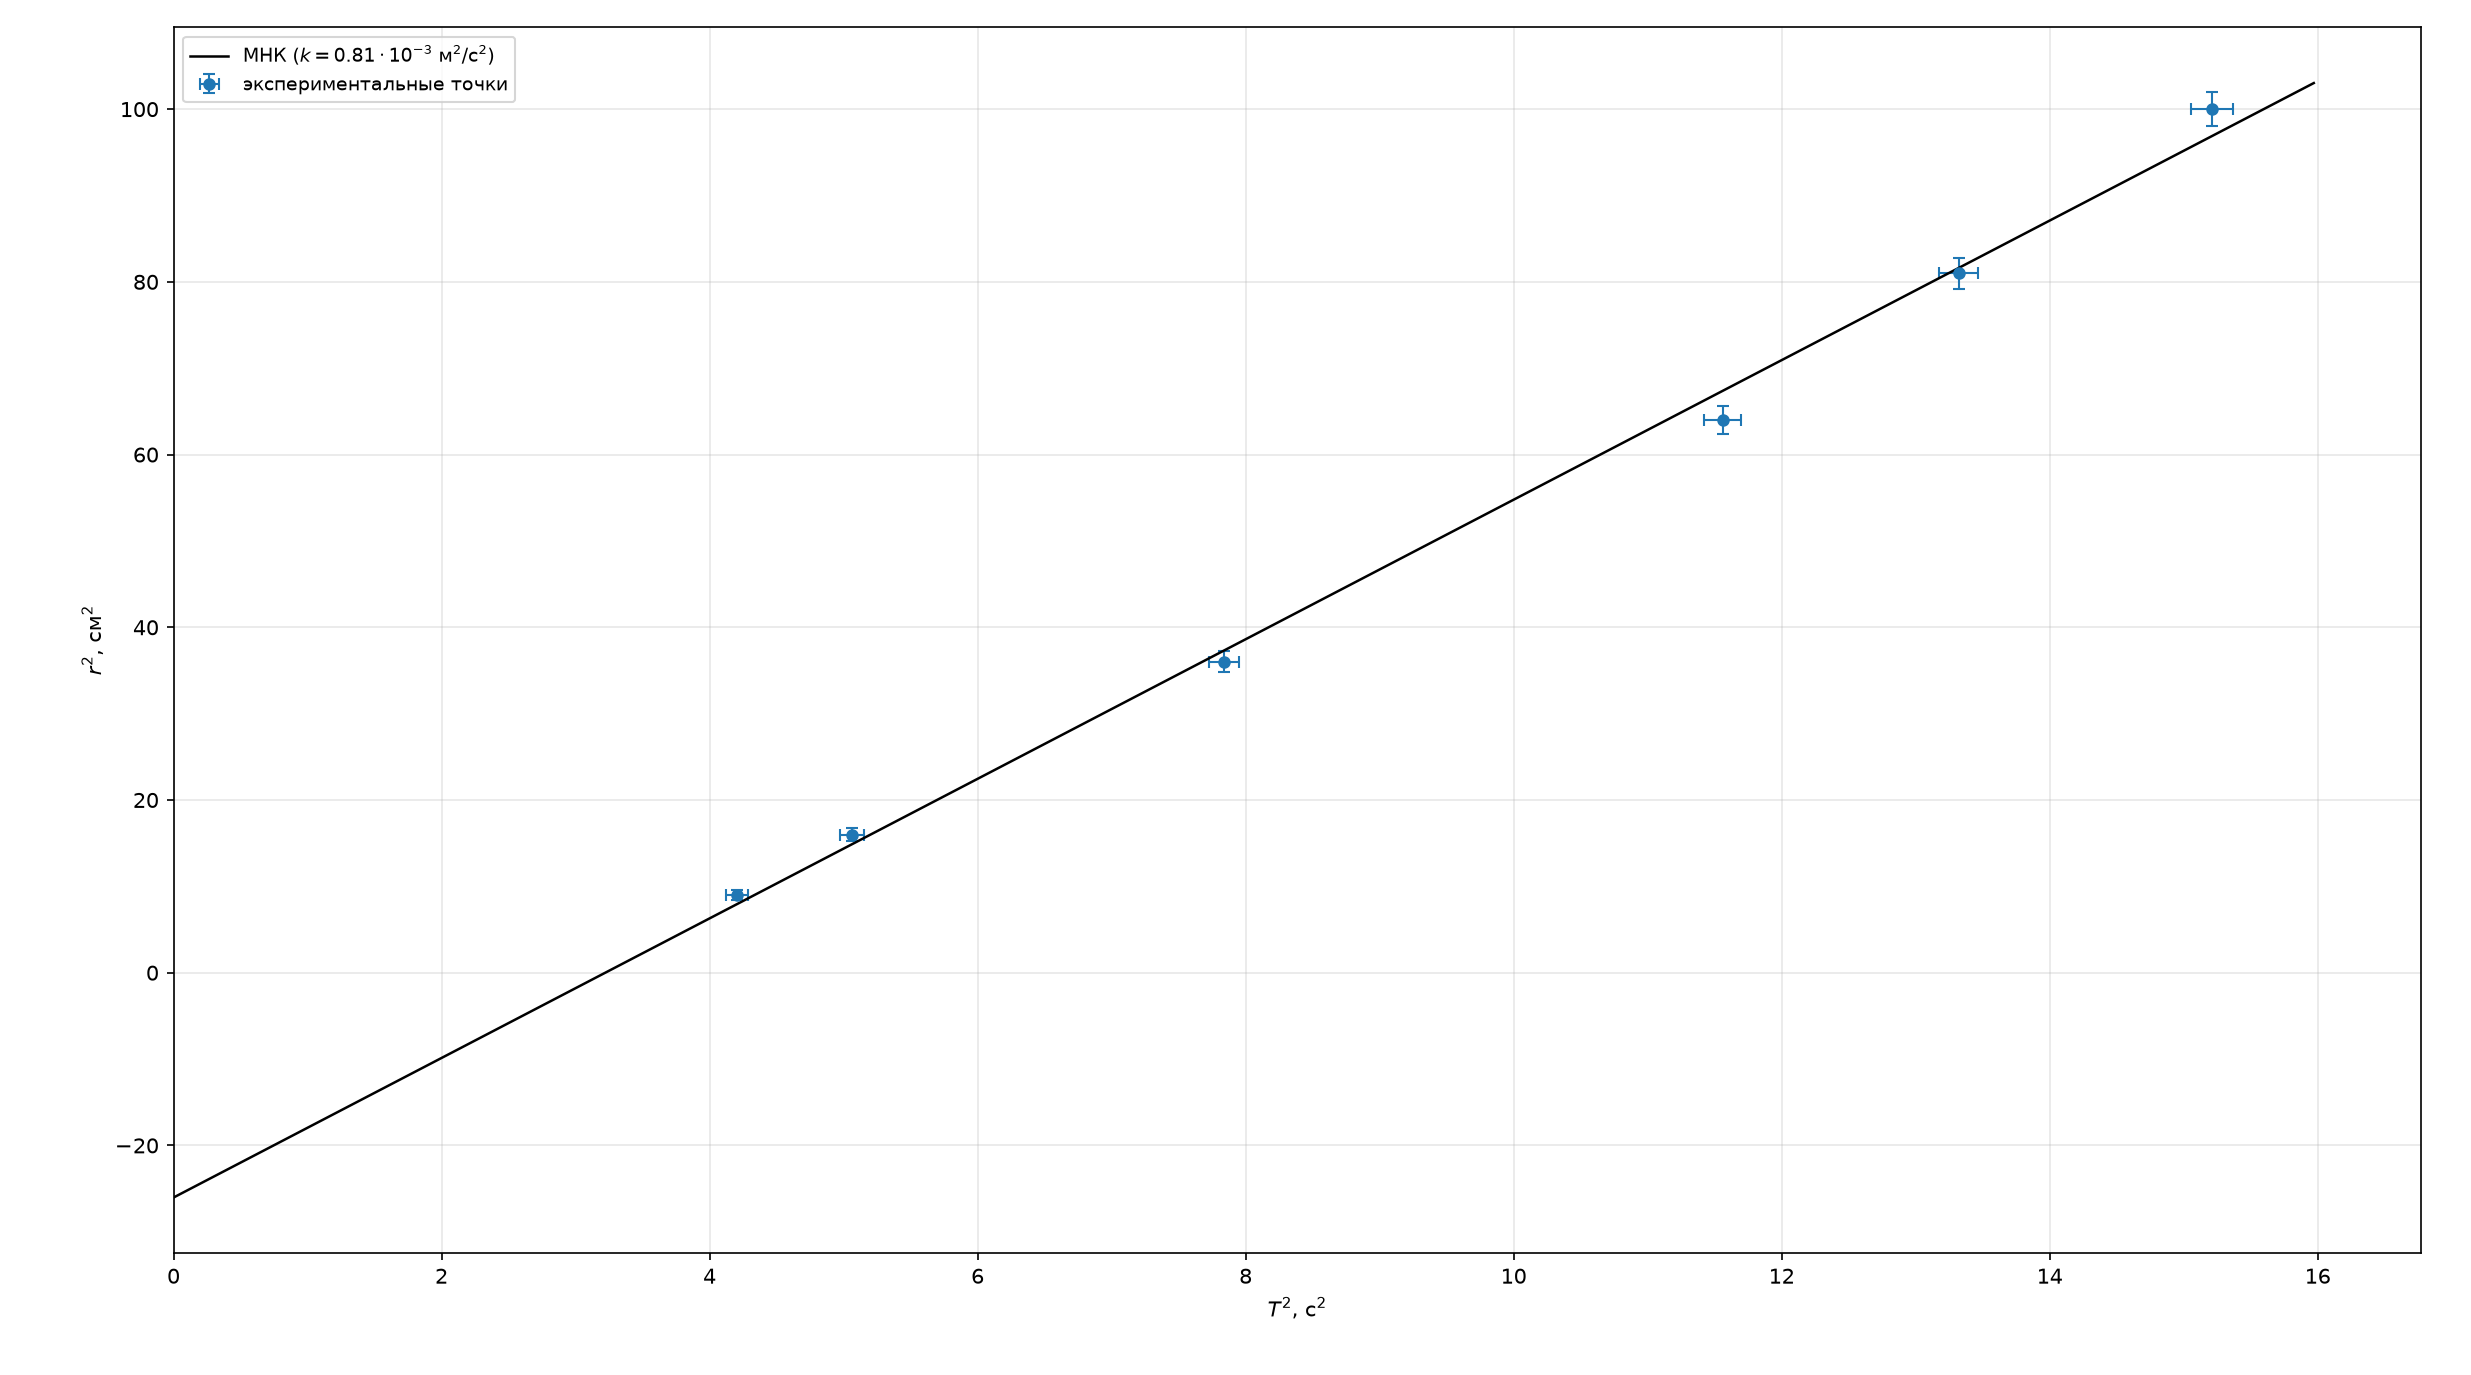
\includegraphics[width=0.85\textwidth]{graph_dynamic.png}
        \caption{График зависимости $r^2$ от $T^2$}
        \label{fig:dyn_graph}
    \end{figure}

    \item Коэффициент наклона графика и его случайную погрешность определим по формулам МНК ($N=6$):
    \[
        k = \frac{\langle T^2r^2\rangle - \langle T^2\rangle\langle r^2\rangle}{\langle T^4\rangle - \langle T^2\rangle^2} = 16.48\cdot10^{-3}~\text{м}^2/\text{с}^2,
    \]
    \[
        \varepsilon_k^{\text{случ}} = \frac{1}{k\sqrt{N-2}}\sqrt{\frac{\langle r^4\rangle - \langle r^2\rangle^2}{\langle T^4\rangle - \langle T^2\rangle^2} - k^2} = 2.1\%,
        \qquad
        \varepsilon_k^{\text{сист}} = 2\sqrt{\varepsilon_T^2 + \varepsilon_r^2} = 2.5\%,
    \]
    \[
        \varepsilon_k = \sqrt{\left(\varepsilon_k^{\text{случ}}\right)^2 + \left(\varepsilon_k^{\text{сист}}\right)^2} = 3.3\%.
    \]
    Итого $k = (16.48 \pm 0.54)\cdot10^{-3}$ м$^2$/с$^2$.

    \item При подсчёте погрешности $f$ учтём, что $\varepsilon_m \ll \varepsilon_k$. Из формулы \eqref{eq:T2} получаем
    \[
        f = (2\pi)^2(m_1+m_2)\,k = (2.45 \pm 0.08)\cdot10^{-2}~\text{Н}\cdot\text{м/рад}, \qquad \varepsilon_f \approx \varepsilon_k = 3.3\%.
    \]

    \item Зная геометрические параметры проволоки и найденный модуль кручения $f$, найдём модуль сдвига $G$ по формуле \eqref{eq:G}:
    \[
        G = \frac{32\,l}{\pi d^4}\,f = 81.5~\text{ГПа}, \qquad
        \varepsilon_G = \sqrt{\varepsilon_f^2 + \varepsilon_l^2 + 16\varepsilon_d^2} = \sqrt{\left(3.3\%\right)^2 + \left(0.1\%\right)^2 + \left(8.0\%\right)^2} = 8.7\%.
    \]
    Получаем итоговое значение модуля сдвига: $G = (81.5 \pm 7.1)$ ГПа, то есть $G \approx 82$ ГПа.

    \item Полученное значение хорошо согласуется с табличными значениями модуля сдвига металлов (для стали $\approx 80$ ГПа). Диаметр проволоки входит в $G$ в четвёртой степени, поэтому 
    основная погрешность связана именно с измерением диаметра. Полученный результат подтверждает, что проволока изготовлена из стали.
\end{itemize}

\section{Выводы}

В результате эксперимента получены значения модуля кручения и модуля сдвига двумя методами.

Статическим методом для стержня: $f = (5.83 \pm 0.04)$ Н$\cdot$м/рад, $G = (80.1 \pm 2.7)$ ГПа ($\varepsilon_G = 3.4\%$). Полученное значение совпадает с табличным для стали ($G\approx 80$ ГПа).

Динамическим методом для проволоки: $f = (2.45 \pm 0.08)\cdot10^{-2}$ Н$\cdot$м/рад ($\varepsilon_f = 3.3\%$). Период колебаний не зависит от амплитуды,
затуханием можно пренебречь, зависимость $r^2(T^2)$ линейна. Модуль сдвига по измеренным геометрическим параметрам проволоки получился $G = (81.5 \pm 7.1)$ ГПа, что  согласуется с табличным значением для стали.

\end{document}